\subsection{OpenCV ORB implementācija}
%~ \subsubsection{OpenCV ORB implementācija}
OpenCV biblotēka\cite{OpenCV-src} piedāvā ORB algoritma implementāciju.
Šī implementācija ir pielāgota secīgai izpildei CPU platformai,
bet tā ir pilnībā skalāra un nesatur būtiskus platformas specifiskus
ātrdarbības uzlabojumus (neskaitot \ref{sec:fast-ocv}~nod.~apskatīto
OpenCV FAST implementāciju, kas izmanto SSE2 SIMD instrukcijas).
rBRIEF salīdzināšanas pāri ir kodā definētas konstantes un
OpenCV nesatur ne saskarnes atbalstu, ne rīkus jaunas salīdzināšanas pāru 
kopas ģenerēšanai ar \ref{sec:rbrief-def}~nodaļā aprakstīto mašīnmācīšanās
metodi.

Rublē~u.c.\cite{ORB}, izstrādājot ORB, diskretizē virziena leņķi $\theta$ ar soli
$\frac{2\pi}{30}$ un aprēķina rBRIEF salīdzināšanas pāru koordinātas katrai no
$\theta$ ieņemamajām vērtībām, izveidojot apjomīgu
,,uzmeklēšanas datubāzi'' (\termEn{look-up table}).
OpenCV šo risinājumu nerealizē, tā vietā --- katra raksturpunkta
deskriptora
salīdzināšanas pāru punktu koordinātas tiek pārrēķinātas 
izmantojot rotācijas matricu kā definēts \eqref{eq:rbrief}~\cite{OpenCV-src}.

OpenCV ORB implementācija testos uzrādīja reāla laika spējīgu
apstrādes ātrumu --- virs 30 kadriem sekundē --- trim no četrām testētajām
ierīcēm (sk.~pielikumu~\ref{appx:test4}).
Salīdzinājums ar GPU implementāciju seko nākamajā (\ref{sec:orb-ocv-cl})
apakšnodaļā.

%~ \subsubsection{OpenCV ORB implementācijas OpenCL versija}
\subsubsection{OpenCL versija}
\label{sec:orb-ocv-cl}
OpenCV bibliotēka piedāvā arī OpenCL ORB versiju izpildei
GPU~\cite{OpenCV-src}. GPU implementācijas galvenā atšķirība no CPU versijas 
ir izpildes pavedienu izveide elementu apstrādei, bet, citādi,
algoritma implementācijas uzbūve ir identiska ar CPU implementāciju.
ORB algoritma OpenCL versijas izpildi var izdalīt vairākos etapos, kuri
uzskaitīti \ref{tbl:orb-ocl-steps}~tabulā.
\begin{table}[thb]\small
	\centering
	\caption{ORB GPU implementācijas izpildes etapi.}
	\label{tbl:orb-ocl-steps}
	\vspace{4pt}
	\begin{tabular}{clcl}
		\toprule
		\textbf{Nr.} & \textbf{Darbība} & $N_e$ & \textbf{Pavediena apstrādājamā vienība}\\
		\midrule
		1. & Attēlu piramīdas izveide & $N_L$ & Rezultējošā attēla pikselis\\
		2. & FAST9 punktu klasifikācija & $N_L$ & Attēla pikselis\\
		3. & FAST9 lokālo maksimumu atlase & $N_L$ & Raksturpunkts\\
		4. & Atlase pēc Harisa stūra mēra & 1 & Raksturpunkts\\
		5. & Intensitāšu centroīdu noteikšana & 1 & Raksturpunkts\\
		6. & Attēlu Gausa filtrēšana & $N_L$ & Rezultējošā attēla pikselis\\
		7. & rBRIEF deskriptoru aprēķins & 1 & Raksturpunkts\\
		\bottomrule
	\end{tabular}
	\begin{minipage}{0.6\linewidth}
		\noindent Apzīmējumi:\\
		$N_e$ --- etapa apakšprogrammas izsaukumu skaits\\
	\end{minipage}
\end{table}

Lai gan GPU teorētiskais skaitļošanas jaudas maksimums ir ievērojami lielāks
nekā CPU, šī ORB implementācija uzrādīja zemus ātrdarbības rādītājus testos
(sk.~\ref{fig:test4-data-text}~att.).
\begin{figure}[tbh]
	\centering
	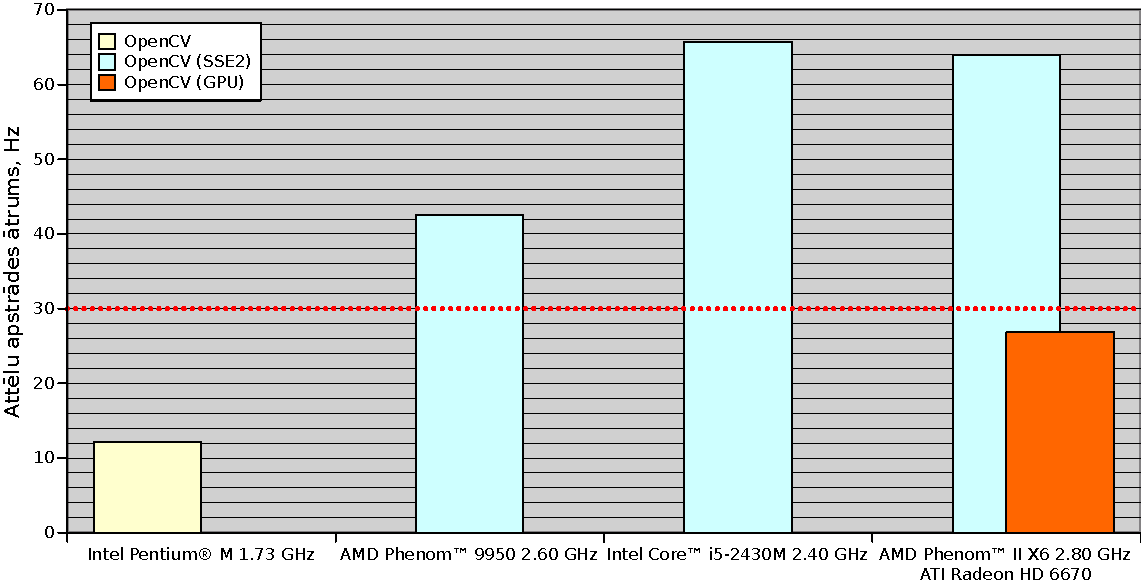
\includegraphics[width=0.9\linewidth]{chart-orb}
	\caption{Ātrdarbība OpenCV ORB implementāciju variantiem dažādās ierīcēs.}
	\label{fig:test4-data-text}
\end{figure}
Autors to skaidro ar nekorektu implementācijas modeli,
nevis platformas veiktspējas trūkumu.
Implementācijas \ref{tbl:orb-ocl-steps} tabulā uzskaitītie etapi,
ir atsevišķas OpenCL apakšprogrammas. Izsaucot OpenCL apakšprogrammu, datus
ir nepieciešams pārvietot uz GPU lokālo atmiņu (video atmiņu)~\cite{OpenCL-book}.
Ņemot vērā, ka katra no implementācijas apakšprogrammām izmanto attēla datus,
un vairums tiek izsauktas vairākkārtīgi, rezultātā vairums laika tiek patērēts
liekai datu pārraidei, šajā laikā skaitļošanas resursiem esot dīkstāvē.

Autora priekšlikums šīs problēmas risinājumam ir realizēt visu algoritmu
vienā OpenCL apakšprogrammā.


